\begin{frame}
\frametitle{CUBIC: default congestion control today}
    \begin{itemize}
    \item default in Linux (since 2006), OS X (since 2014), Windows (since 2019)
        \begin{itemize}
        \item sysadmin has other options they can configure
        \item can be changed on connection-by-connection basis
        \end{itemize}
    \item includes improvements to recovery we'll talk about later
    \item but mostn notably has non-additive increase
    \end{itemize}
\end{frame}

\begin{frame}
    \frametitle{increase intuition}
    \begin{itemize}
        \item `standard' TCP basically has two increase algorithms:
        \item slow start --- quickly explore window sizes
        \item congestion avoidance --- slowly probe for maximum
        \vspace{.5cm}
        \item abrupt transition between these is suspect
            \begin{itemize}
            \item should have gradual exploration $\rightarrow$ fine-tuning switch
            \end{itemize}
        \item heuristic for when to use slow start-style is suspect
            \begin{itemize}
            \item half way from last loss $\approx$ guess?
            \end{itemize}
    \end{itemize}
\end{frame}

\begin{frame}
    \frametitle{CUBIC increase algorithm}
    \begin{itemize}
    \item big idea: faster increase when further away from window size of last loss
        \begin{itemize}
        \item cubic function with saddle point at that window size
        \item function parameterized by time since loss
        \end{itemize}
    \item intuition for `steady state':
        \begin{itemize}
        \item guess correct window size is close to last loss
        \item quickly get to around that window size
        \item search slowly/precisely around that size to fine tune size
        \end{itemize}
    \item intuition for non-steady state:
        \begin{itemize}
        \item try to quickly probe for roughly how small/big it is
        \item worry about getting more precise size on later `pass'
        \end{itemize}
    \end{itemize}
\end{frame}


\begin{frame}{}
\begin{tikzpicture}
\node (pic) {
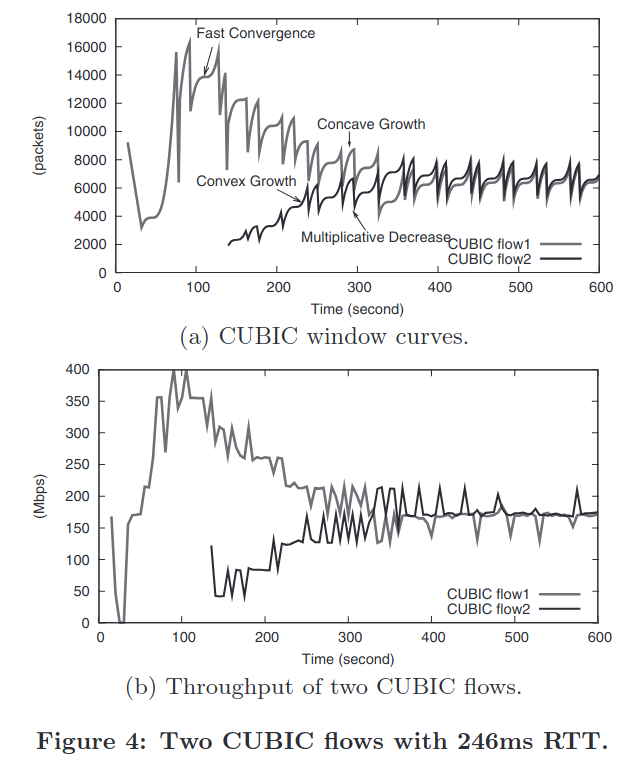
\includegraphics[height=\textheight]{../congest/cubic-fig4}
};
\node[anchor=north west,font=\tiny] at (pic.north east) {
from Ha, Rhee, and Xu, ``CUBIC: A New TCP-Friendly High-Speed TCP Variant''
};
\end{tikzpicture}
\end{frame}

\begin{frame}
    \frametitle{other CUBIC changes}
    \begin{itemize}
        \item different multiplicative decrease factor (divide by 1.4)
    \end{itemize}
\end{frame}
